\chapter{Thử nghiệm và đánh giá}
\section{Triển khai chạy thử nghiệm trên cloud}
Trong đồ án này, em sử dụng Microsoft Azure làm nhà cung cấp dịch vụ
cloud và sử dụng Azure Kubernetes Service để triển khai các server.
Kiến trúc tổng quan của hệ thống như hình sau:
\begin{figure}[H]
\centering
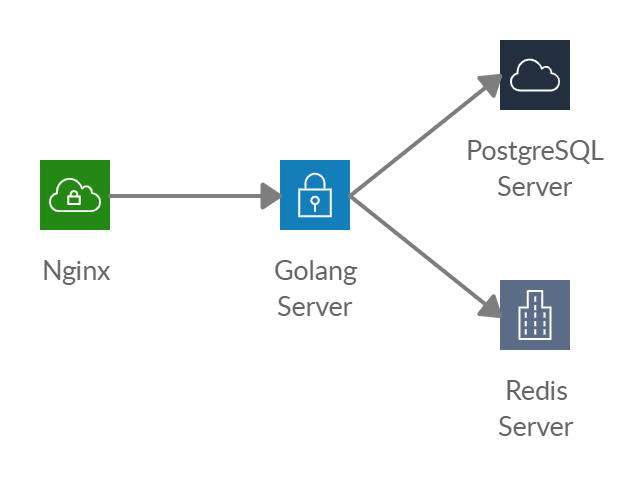
\includegraphics[width=10cm]{images/architecture.png}
\caption{Kiến trúc tổng quan của hệ thống}
\end{figure}
Trong đó:
\begin{itemize}[topsep=0ex]
\item Nginx: sử dụng để làm web server trả về các file tĩnh html và js khi
ứng dụng được mở lên lần đầu, đồng thời được sử dụng làm Reverse Proxy đến
Golang Server cho các Rest API.

\item Golang Server: web server cho các Rest API từ trình duyệt gửi lên
thông qua AJAX.

\item PostgeSQL Server: cơ sử dữ liệu quan hệ của hệ thống.

\item Redis Server: lưu trữ dữ liệu của các phiên làm việc (session).
\end{itemize}

Còn để triển khai lên AKS, em đã sử dụng những thành phần sau:
\begin{figure}[H]
\centering
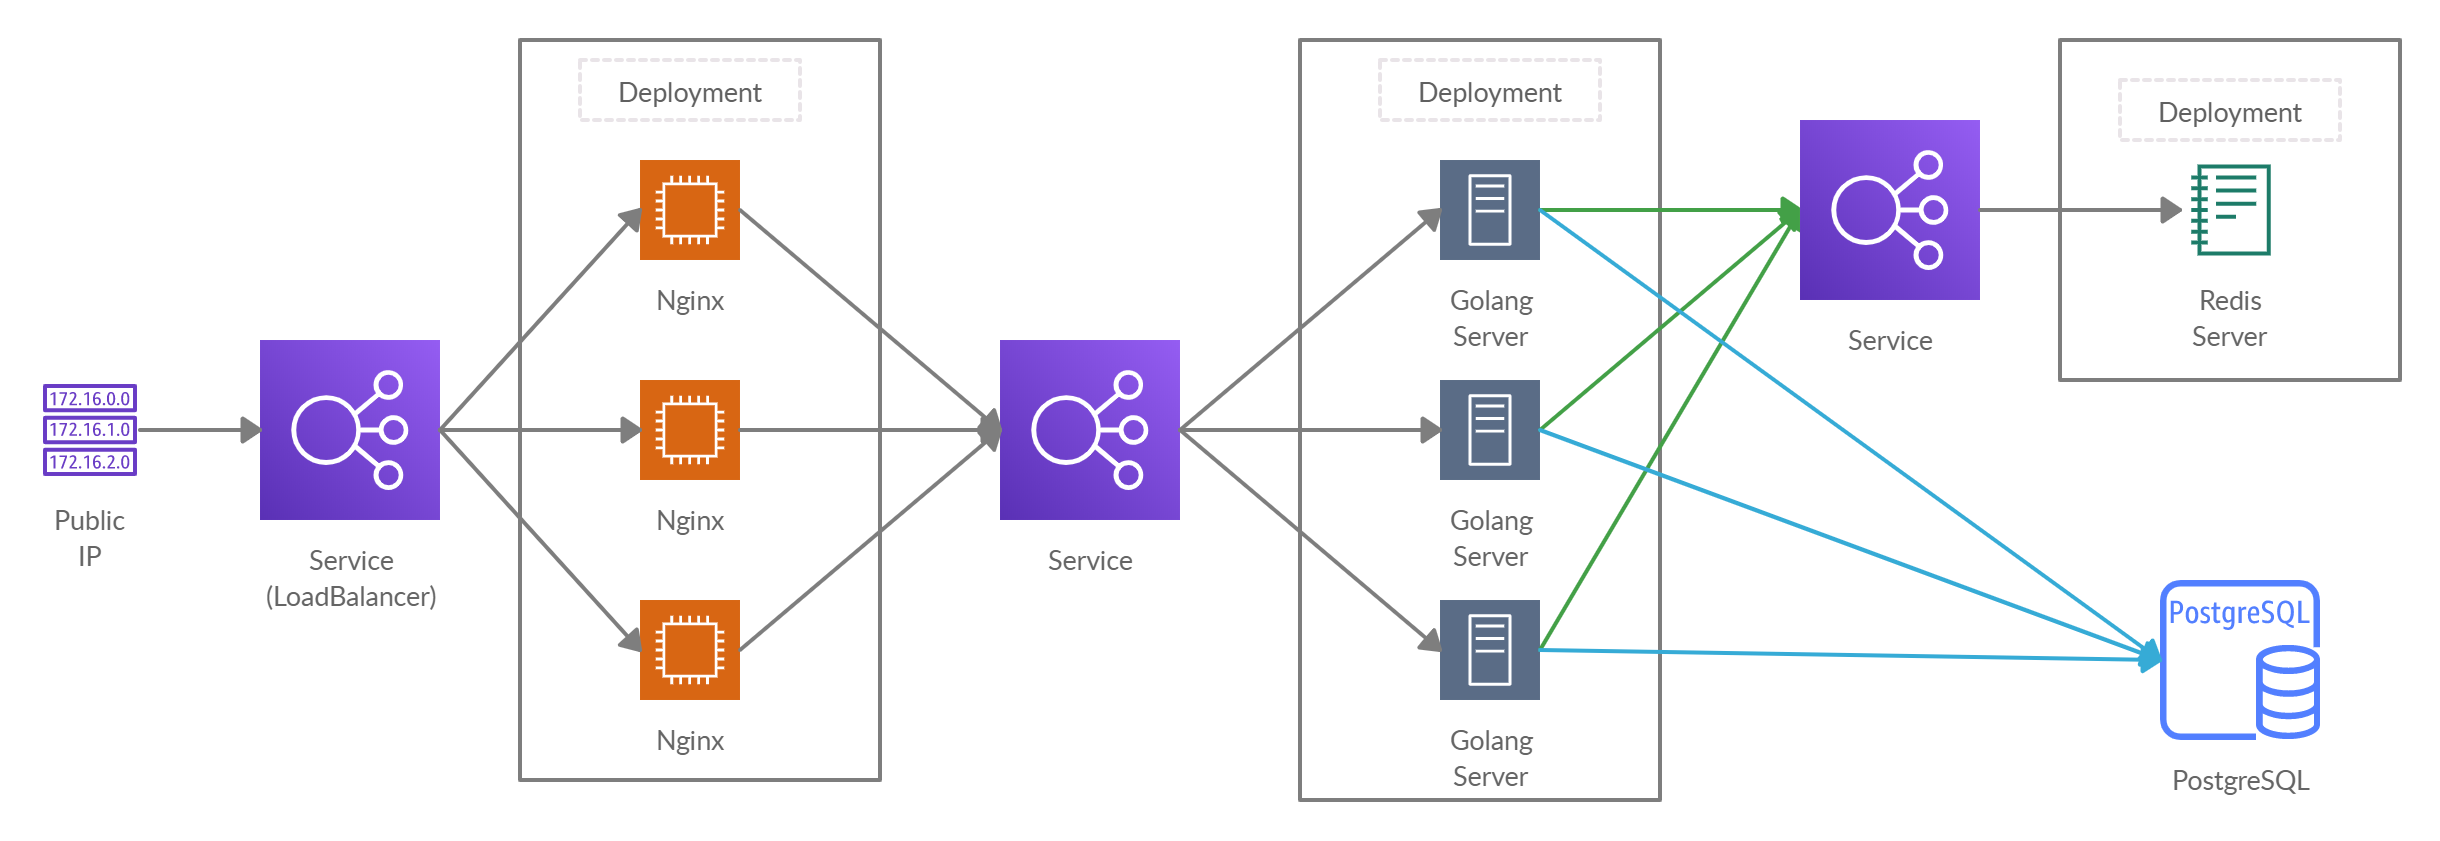
\includegraphics[width=\textwidth]{images/deploy.png}
\caption{Triển khai lên Azure Kubernetes Service}
\end{figure}

Kết quả sau khi triển khai là hệ thống có thể truy cập được
từ địa chỉ public IP.

\section{Kiểm thử hiệu năng (performance testing)}
\section{Kiểm thử sức chịu tải (stress testing)}
